\documentclass[12pt,openright,twoside,a4paper]{book}
\usepackage{hyperref}
\usepackage[T1]{fontenc}
\usepackage[utf8]{inputenc}
\usepackage[english]{babel}
\usepackage{amsmath}
\usepackage{amssymb}
\usepackage{caption}
\usepackage{graphicx}
\usepackage{booktabs}
\usepackage{textcomp}
\usepackage{amsfonts}


% permette di inserire le note a margine
\usepackage{marginnote}


\begin{document}

\frontmatter

\tableofcontents

\chapter{Introduction}

\mainmatter

\chapter{The Wishart Distribution}

\section{Definition}

The \textit{wishart distribution} $ W_p(n, \Sigma)$ is a probability distribution of random nonnegative-definite $p\times p$ matrices that is used to model random covariance matrices.

The parameter $n$ is the number of degrees of freedom, and $\Sigma$ is a nonnegative-definite symmetric $p\times p$ matrix, called the \textit{scale matrix}.


\textit{Def.} Let $X_1...X_n$ be independent $N_p(0,\Sigma)$ distribuited vectors, forming a data matrix $p\times n$, $X=[X_1...X_n]$.
The distribution of  a $p\times p$, $M=XX'=\Sigma^n_{i=1}X_iX_i'$ \textit{random matrix}  is a Wishart distribution. \cite{AMS}

We have then by definition:

\begin{equation}
M\sim W_p(n, \Sigma)\sim\Sigma^n_{i=1}X_iX_i' \qquad X_i\sim N_p(0,\Sigma)   
\label{wsim}
\end{equation}


so that $M\sim W_p(n, \Sigma)$  is the distribution of a sum of $n$ rank-one matrices defined by independent normal $X_i \in R^p$ with $E(X)=0$ and $Cov(X)=\Sigma$.

In particular, it holds for the present case:

\begin{equation}
E(M)=nE(X_iX_i') = nCov(X_i) = n\Sigma
\end{equation}

\section{PDF Computation for Invertible $\Sigma$}

In general, any $X\sim N(\mu,\Sigma)$ can be represented as
\begin{equation}
X=\mu + AZ,\quad Z\sim N(0,I_p)
\end{equation}
so that
\begin{equation}
\Sigma= Cov(X) = A Cov(Z)A' = AA'
\label{covZ}
\end{equation}


The easiest way to find $ A$ in terms of $\Sigma$ is the LU-decomposition, which finds a unique lower diagonal matrix $A$ with $A_{ii} \geqslant 0 $ such that $AA' = \Sigma$.

Then by \ref{wsim} and \ref{covZ}, with $\mu=0$ we have:

\begin{equation}
W_p(n, \Sigma)\sim \sum_{i=1}^n(AZ_i)(AZ_i)'\sim A(\sum_{i=1}^nZ_iZ_i')A'\sim AW_p(n)A'
\end{equation}
where $Z_i\sim N(0, I_p)$ and $W_p(n)=W_p(I_p,n)$. 

Assuming that  $n\geq p$ and $\Sigma$ is invertible, the density of the random $p\times p $ matrix $M$ in \ref{wsim} can be written \footnote{\textit{Note: $\|\Sigma , N \| = det (\Sigma , M)$}} :

\begin{equation}
f(M, n, \Sigma)=\frac{1}{2^{\frac{np}{2}}\Gamma_p(\frac{n}{2})\|\Sigma\|^{\frac{n}{2}}}\|M\|^{\frac{n-p-1}{2}}exp[-\frac{1}{2}trace(\Sigma^{-1}M)]
\label{Wishart-pdf}
\end{equation} 

so that $f(M, n, \Sigma)=0$ unless $M$ is \textit{symmetric and positive-definite}. \cite{IMS}

Note that in \ref{Wishart-pdf} we define $\Gamma_p(\alpha)$ as the \textit{generalized gamma function} $\Gamma_p(\alpha)=\pi^\frac{p(p-1)}{4}\prod_{i=1}^p\Gamma(\frac{2\alpha+1-i}{2})$

\subsection{Visualizing the Wishart Distribution}

The Wishart distribution is a generalization to multiple dimensions of the \textit{chi-squared distribution}, or in the case of non-integer degrees of freedom, of the \textit{gamma distribution}.

We show as a proof in fig.\ref{Wish-chi2} that for a 1-dimensional and equal to 1 $\Sigma$ scale matrix, the Wishart distribution $W_1(n,1)$ collapses to the $\chi^2(n)$ distribution.

\begin{figure}[!h]
\centering
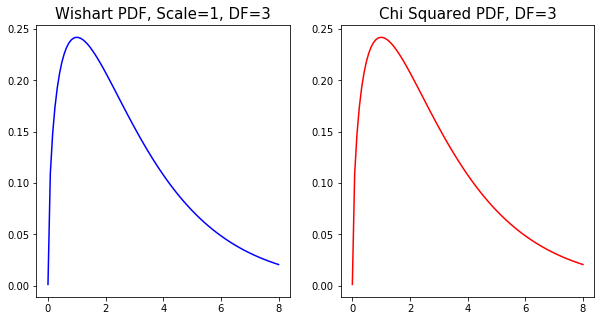
\includegraphics[scale=0.37]{wish-chi}
\caption{\textit{Monodimensional Wishart Distribution and $\chi^2(n)$ distribution comparison}}
\label{Wish-chi2}
\end{figure}

Save for this simple case, being the Wishart a distribution over matrices, it is a generally hard task to visualize it as a density function.

We can however sample from it and use the eigenvectors and eigenvalues of the resulting sampled matrix to define an ellipse.

An example of this technique is shown in fig.\ref{Wish-eig}. A set of five sampled matrices is drawn for each plot. While the parameter $n=2$ (\textit{degrees of freedom}) is the same for both the samplings shown, a different \textit{scale matrix} $\Sigma$ is used for each plot.

Note that for $\Sigma=I_2$ (left plot in fig.\ref{Wish-eig}) the sample would look \textit{on average} like circles.

\begin{figure}[!h]
\centering
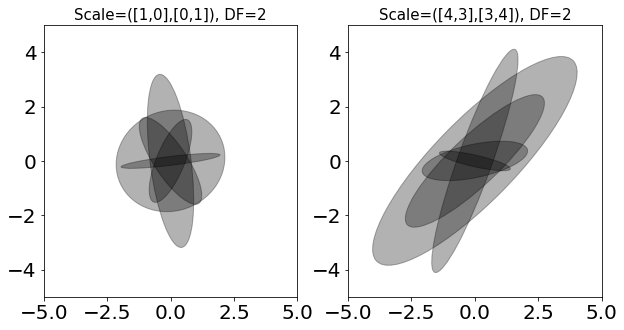
\includegraphics[scale=0.37]{wisheig-df2}
\caption{\textit{Plot of eigenvalue and eigenvectors defined ellipses, drawn from different scale matrix defined Wishart-sampled distribution. }}
\label{Wish-eig}
\end{figure}

\section{The Wishart Distribution in Bayesian Conjugate Prior Analysis}

An important use of the Wishart distribution is as a conjugate prior for \textit{multivariate normal sampling}. We now recall some basics concepts about Bayesian inference and prediction in order to show the application of the Wishart in those fields.

\subsection{Bayesian Inference and Priors Distributions}

The distinctive feature of the Bayesian approach underlies in its way of defining probability.

Probability is treated as \textit{belief} and not as \textit{frequency}, thus introducing a fundamental difference between the Bayesian and the \textit{frequentist} approach and shifting the goal toward the analysis and statement of a \textit{belief} \cite{SML}.
\\[12pt]
We can sum up the process of Bayesian inference as follows:
\begin{itemize}
\item A probability density called \textit{prior distribution} $\pi(\theta)$ is chosen, expressing the \textit{beliefs} about a parameter $\theta$ before any data are seen.
\item A statistical model $p(x\mid \theta)$ is chosen, which must reflect the beliefs about $x$ given $\theta$.
\item After observing the data $D_n=[X_1...X_n]$, the beliefs is updated and the \textit{posterior distribution} $p(\theta\mid D_n)$ is computed.
\end{itemize}

By Bayes' theorem the posterior distribution can be written as 

\begin{equation}
p(\theta\mid X_1...X_n)= \frac{p(X_1...X_n\mid \theta)\pi(\theta)}{p(X_1...X_n)}=\frac{L_n(\theta)\pi(\theta)}{c_n}\propto L_n(\theta)\pi(\theta)
\label{bayest}
\end{equation}

where $L_n(\theta)=\prod_{i=1}^n p(X_i\mid \theta)$ is the likelihood function and the \textit{normalizing constant} $c_n$ is defined as follows:

\begin{equation}
c_n=p(X_1...X_n)=\int p(X_1...X_n\mid \theta)\pi(\theta)d\theta=\int L_n(\theta)\pi(\theta)d\theta
\label{cnorm}
\end{equation}

the normalizing constant is also called the \textit{evidence}.

We now define the general properties of a \textit{conjugate prior}.

If, for a given problem, the posterior distribution $p(\theta\mid X_1...X_n)$ and the prior $\pi(\theta)$ belong to the same family of distribution, they're called \textit{conjugated distributions} and the prior is said to be a \textit{conjugate prior} for the given \textit{likelihood function} $L_n=p(X_1...X_n\mid \theta)$.

A classical example concerns the Gaussian Distribution: the Gaussian family is conjugate to itself (or self-conjugate) with respect to a Gaussian likelihood function: if the likelihood function is Gaussian, choosing a Gaussian prior over the mean will ensure that the posterior distribution is also Gaussian \cite{CBA}.

Considering the general problem of inferring a distribution for a parameter $\theta$ given some observations $D_n=[X_1...X_n]$ and referring to theorem \ref{bayest}, by which we let the likelihood function be considered fixed as it is usually well-determined from a statement of the data-generating process,  it is clear that different choices of the prior distribution $\pi(\theta)$ may make the integral in \ref{cnorm} more or less difficult to compute.
The product $L_n(\theta)\pi(\theta)$ will also be influenced, gaining the possibility to take one algebraic form or another.

If for certain choices of the prior the posterior has the same algebraic form as the prior, those choices are said to yield a \textit{conjugate prior}.

It is then possible to state that a conjugate prior is an algebraic convenience giving a closed-under-sampling-form expression for the posterior.

\subsection{The Wishart Conjugate Prior}

We now show how the Wishart Distribution is correlated to the\textit{Inverse Gamma Distribution} in a multidimensional setting, by  considering a Gaussian model with known mean $\mu$, so that the free parameter is the variance  $\sigma^2$, as in \cite{SML}.

The likelihood function is defined as follows:

\begin{equation}
p(X_1...X_n\mid \sigma^2)\propto (\sigma^2)^{-\frac{n}{2}}exp(-\frac{1}{2\sigma^2}n \overline{(X-\mu^2)}) , \qquad \overline{(X-\mu^2)}=\frac{1}{n}\sum_{i=1}^n(X_i-\mu)^2
\label{gausslike}
\end{equation}
\\[12pt]

The conjugate prior is an inverse Gamma distribution. Recall that $\theta$ has an inverse Gamma distribution with parameters $(\alpha,\beta)$   when $\frac{1}{\theta}\sim Gamma(\alpha,\beta)$.

The density is then bound to take the form 

\begin{equation}
\pi_{\alpha,\beta}(\theta)\propto \theta^{-(\alpha+1)}e^{-\frac{\beta}{\theta}}
\end{equation}

Using this prior, the posterior distribution of $\sigma^2$ is given by

\begin{equation}
p( \sigma^2 \mid X_1...X_n)\sim InvGamma(\alpha + \frac{n}{2}, \beta + \frac{n}{2} \overline{(X-\mu^2)})
\end{equation}

An alternative way of parameterization of the prior is given by the \textit{Inverse Scaled $\chi^2$ Distribution}, whose density is defined as

\begin{equation}
\pi_{\nu_0, \sigma_0^2}\propto \theta^{-(1+ \frac{n_0}{2})}exp(-\frac{\nu_0 \sigma_0^2}{2\theta})
\end{equation}

Under this kind of parameterization of the prior, the posterior takes the form

\begin{equation}
p(\sigma^2 \mid X_1...X_n)\sim ScaledInv\chi^2(\nu_0+n, \frac{\nu_0 \sigma_0^2}{\nu_0 + n} + \frac{n(X-\mu^2)}{\nu_0 + n})
\end{equation}

In the multidimensional setting, the inverse Wishart takes the place of the inverse Gamma.

It has already been stated that the Wishart distribution is a distribution over \textit{symmetric positive semi-definite} $d\times d$ matrices $W$. A more compact form of the density is given by

\begin{equation}
\pi_{\nu_0, S_0}(W)\propto \mid W\mid ^{\frac{(\nu_0-d-1)}{2}}exp(-\frac{1}{2}trace(S_0^{-1}W)), \qquad \mid W\mid=det(W)
\end{equation}

where the parameters are the degrees of freedom $\nu_0$ and the positive-definite \textit{scale matrix}
$S_0$.

If $W^{-1}\sim Wishart(\nu_0, S_0)$ we can then state that $W$ has an \textit{Inverse Wishart Distribution}, whose density has the form
\begin{equation}
\pi_{\nu_0, S_0}(W)\propto \mid W\mid ^{-\frac{(\nu_0+d+1)}{2}}exp(-\frac{1}{2}trace(S_0W^{-1})), \qquad \mid W\mid=det(W)
\end{equation}

Let $X_1...X_n$ be $N(0,\Sigma)$ distributed observed data. Then an inverse Wishart prior multiplying the likelihood $p(X_1...X_n\mid \Sigma)$ yields

\begin{equation}
\begin{aligned}
p(X_1...X_n\mid \Sigma)\pi_{\nu_0, S_0}(\Sigma)\propto \\[10pt]
 \mid\Sigma \mid ^{-\frac{n}{2}}exp(-\frac{n}{2}trace(\overline{S} \Sigma^{-1}) \mid \Sigma\mid ^{-\frac{(\nu_0+d+1)}{2}}exp(-\frac{1}{2}trace(S_0\Sigma^{-1})) \\[10pt]  
=  \mid \Sigma\mid ^{-\frac{(\nu_0+d+n+1)}{2}}exp(-\frac{1}{2}trace((n\overline{S}+S_0)\Sigma^{-1}))
\end{aligned}
\end{equation}

where $\overline{S}$ is the \textit{empirical covariance} $\overline{S}=\frac{1}{n}\sum_{i=1}
^nX_iX_i^T$.

Thus, a posterior with the form

\begin{equation}
p(\Sigma\mid X_1...X_n)\sim InvWishart(\nu_0+n, n\overline{S}+S_0)
\end{equation}

is obtained.

Analogally, it can be stated that for the inverse covariance (\textit{precision}) matrix $\Sigma^{-1}$ the conjugate prior is a Wishart distribution.

\chapter{The WISDoM Multiple Order Classifier}

In this section, the classification method implemented and used on the ADNI2 and ABIDE databases is described, both in an analytical and technical way.

The \textit{"distance"} used to train the classifier is defined as well as the \textit{feature transformation} undergone by the each of the subject analyzed.

The general pipeline and the validation pipeline are then discussed while also introducing an example of possible parallelization for performance enhancing.

\section{Wishart Sampling and Log-Likelihood Ratio Distance}

Considering what has been said in the last section, using the Wishart distribution to model and sample the elements of a wide range of problems follows naturally.

As a matter of fact, every calssification problem whose elements take the form of \textit{symmetric positive-definite} matrices can be approached with the method we are about to discuss.

The main idea for the \textit{WISDoM Classifier} is to use the \textit{free parameters} of the Wishart distribution (the scale matrix $S_0$ and the number $n$ of the degree of freedom, as shown in \ref{Wishart-pdf}) to compute an estimation of the distribution for a certain class of elements, and then assign a single element to a given class by computing some sort of distance between the element being analyzed and the classes.

Furhermore, if we assume that the matrices are somehow representative of the \textit{features} of the system studied (i.e. covariance  matrices might be taken into account), a score can be assigned to each feature by estimating the weight of said feature in terms of \textit{Log Likelihood Ratio}.

In other words, a score can be assigned to each feature by analyzing the variation in terms of \textit{LogLikelihood} caused by the deletion of it. 

If the deletion of a feature causes significant increase (or decrease) in the \textit{LogLikelihood} computed with respect to the \textit{estimated distributions} for the classes, it can be stated that said feature is highly representative of the system analyzed.

It is now clear that the simplest usable objects to estimate the distribution for a class and to represent its elements is the \textit{covariance  matrix}. Further proofs for this statement will be given later on.

Thus, the aim of the WISDoM classifier is not only to assign a given element to the optimal class, but also to identify the features with the highest \textit{"weights"} in the decision process.

\subsection{Computing the Estimated Distribution}

Let us briefly recall the parametrization of the Wishart Distribution in order to clearly define the application conditions for classification problems.

Let $X_1...X_n$ be independent $N_p(0,\Sigma)$ distributed vectors, forming a data matrix $p\times n$, $X=[X_1...X_n]$.
The distribution of  a $p\times p$, $M=XX'=\Sigma^n_{i=1}X_iX_i'$ \textit{random matrix}  is a Wishart distribution with parameters $W_p (n, S_0 )$. In the previous chapter (\ref{Wishart-pdf}) it has been proved that for normal distributed data, for $S_0=\Sigma$, a distribution of \textit{random covariance matrices} is obtained.

In a similar fashion, if a good choice for the scale matrix $S_0$ is made for a given class, a representative distribution for the class can be estimated and samples can be drawn from it.

\textit{Covariance matrices} are a good choice, although not limiting as long as the matrices are symmetric and positive-definite, both for the way they represent a system and for the property that \textit{the mean of a set of covariance matrices is a covariance matrix}. 

If each element of a given class $C$ is represented by a covariance matrix $\Sigma$ of its features, this property allows us to estimate a distribution for the class by choosing $S_0=\hat{\Sigma}_C=\frac{1}{N}\sum_{i=1}^N \Sigma_i$.

The other necessary parameter for the estimation is the \textit{degrees of freedom n}.

Assume that an $X_i=(x_1, ..., x_p)$ vector of $p$ features is associated to each element $i$ of a given class, while having $n$ observation of said vector. The covariance matrix $\Sigma_i$ computed over the $n$ observations will represent the "interactions" between the features of element $i$.

The degrees of freedom  $n$ of the Wishart distribution are then given by the number of times $X_i$ is observed.

Let us introduce an example tied to \textit{functional MR brain imaging } in order to further clarify the concepts being introduced. 

An image of patient $i$'s brain is acquired; as usual these images are divided in a certain number $p$ of zones (voxel, pixel etc.), each zone being sampled $n$ times over a given time interval in order to observe a certain type of brain activity and functionality.

It is now clear that the features contained in vector $X_i=(x_1,..,x_p)$ associated to patient $i$ are indeed the zones chosen to divide $i$'s brain image, each zone having been sampled $n$ times during an acquisition interval.

The correlation $p \times p$ matrix $\Sigma_i$ computed for $i$'s observation is then representative of the functional correlation between the $p$ zones of $i$'s brain.

Repeating this procedure for $N$ patients belonging to a known class $C$ (i.e. a diagnostic group) and computing the $\hat{\Sigma}_C$ scale matrix for the class as stated before, will allow us to estimate a wishart distribution for that class correlation matrices and draw samples from it.

\vspace{5mm}

The module used for Wishart generation and sampling by the WISDoM calssifier is the \textit{SciPy.Stats.Wishart} module of the \textit{SciPy} Python3.6 library.

Further details on the generation and sampling algorithm used  by the module can be found in \cite{WishGen}.

Some  samples drawn from Wishart distributions computed with different  $5 \times 5$ scale matrices and degrees of freedom are shown in fig.\ref{randmatr}.

\clearpage

\begin{figure}[!h]
\centering
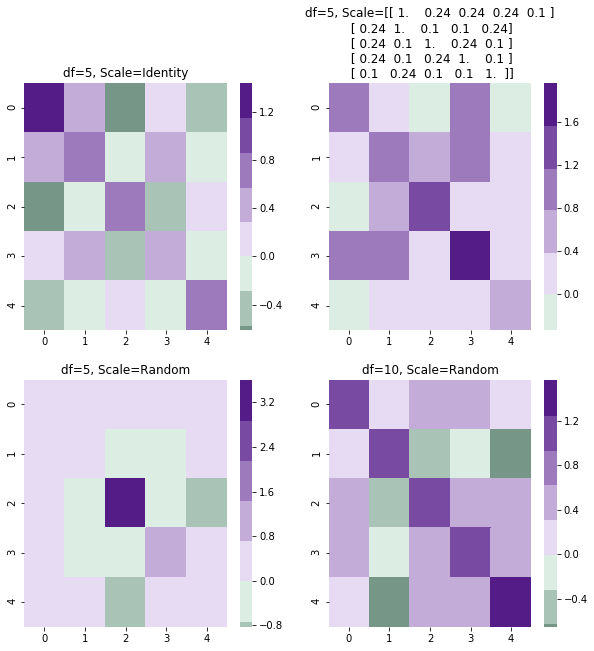
\includegraphics[scale=0.5]{randmatr}
\caption{\textit{Various sampling from different wishart distribution. A diverging heatmap has been chosen to visualize the values of each sample's elements.}}
\label{randmatr}
\end{figure}

\section{Log-Likelihood Ratio Distance}

After the definition of the role of the Wishart distribution in symmetric positive definite matrices' modeling, it is necessary to define some sort of distance between the estimated distribution for a class $C$ and its hypotetical elements.

As stated before, this will be done in terms of both entire matrices and \textit{single features}, in order to achieve optimal classification and exract information about a system's most meaningful components.

\subsection{Complete Matrix Distance}

The scoring system used by the WISDoM Classifier relies on the \textit{logpdf} function from the \textit{SciPy.Stats.Wishart} module in order to compute the LogLikelihood of a matrix $\Sigma_i$ with respect to the Wishart distribution estimated for a class $C$, using $\hat{\Sigma}_C$ as the scale marix.

If a problem concering two given classes $C_A$ and $C_B$ is taken into account, the score assigned to each $\Sigma_i$ upon which the classification decision is based, can be defined as follows:

\begin{equation}
score_{i}= logP_{W}(\Sigma_{i}\mid n, \hat{\Sigma}_{A})-logP_{W}(\Sigma_{i}\mid n,\hat{\Sigma}_{B})
\label{pdf-score}
\end{equation}

Where $\hat{\Sigma}_{A,B}$ are the scale matrix computed for the classes $A,B$ and $ logP_{W}(\Sigma_{i}\mid n, \hat{\Sigma}_{A,B})$ can be seen as the logarithm of the probability of $\Sigma_i$ belonging to the Wishart distribution estimated for one of the two classes $A,B$.

\subsection{Single Feature Distance and Multiple Order Reduction}

The aim of the WISDoM classifier is to further increase the informations obtained about the system's features during the classification.

To do this it is then necessary to introduce some matemathical properties of the symmetric positive deifnite matrices, upon which the method relies.

It will be shown that it is indeed possible to access different orders of information by scaling a matrix $A$ to its \textit{principal submatrices}.

\vspace{5mm}

\textbf{Def.} \textit{Let $A$ be an $n \times n$ matrix. A $k \times k$ submatrix of $A$ formed by deleting $n-k$ rows of $A$, and the same $n-k$ columns of $A$, is called principal submatrix of $A$. The determinant of a principal submatrix of $A$ is called a principal minor of $A$.}

\vspace{5mm}

Note that the definition does not specify which $n-k$ rows and columns to delete, only that their indices must be the same.

Let us introduce a $3 \times 3$ example.

For a general matrix $A_{3\times 3}$ 

\begin{equation}
A=
\begin{bmatrix}
         a_{11} & a_{12} & a_{13} \\
    	    a_{21} & a_{22} & a_{23} \\ 
	    a_{31} & a_{32} & a_{33}  
\end{bmatrix}
\end{equation}

\vspace{5mm}

there are three \textit{first order principal minors}:

\begin{itemize}
\item $\mid a_{11}\mid$ formed by deleting the last two rows and columns
\item $\mid a_{22}\mid$ formed by deleting the first and third rows and columns
\item $\mid a_{33}\mid$ formed by deleting the first two rows and columns

\end{itemize}

There are three \textit{second order principal minors}:

\begin{itemize}
\item 
$\mid\begin{bmatrix}
         a_{11} & a_{12}  \\
    	    a_{21} & a_{22}  \\ 
\end{bmatrix}\mid$ formed by deleting column 3 and row 3

\item
$\mid\begin{bmatrix}
         a_{11}  & a_{13} \\
	    a_{31}  & a_{33}  
\end{bmatrix}\mid$ formed by deleting column 2 and row 2

\item
$\mid\begin{bmatrix}
         a_{22} & a_{23} \\ 
	     a_{32} & a_{33}  
\end{bmatrix}\mid$ formed by deleting column 1 and row 1

\end{itemize}

There's one \textit{third order principal minor}, namely $\mid A\mid$.

\vspace{5mm}

For the sake of completion, we also recall the following definition.

\textbf{Def.} \textit{Let $A$ by an $n\times n$ matrix. The $k^{th}$ order principal sub-matrix of $A$ obtained by deleting the \textbf{last} $n-k$ rows and columns of $A$ is called the $k^{th}$ order \textbf{leading principal submatrix} of $A$, and its determinant is called the  $k^{t}h$ \textbf{order leading principal minor} of A.}
\vspace{5mm}

An imporant property for the principal submatrices of a symmetric positive definite matrix is that \textit{any $(n-k)\times (n-k)$ partition is also symmetric and positive definite.}

It is now clear that such properties can be used to reduce both a class scale matrix $\hat{\Sigma}_C$ and any $\Sigma_i$ matrix, in order to study its deviation from a class's estimated Wishart distribution derived from the deletion of one of its components (the features conatined in vector $X_p$ from which the matrix $\Sigma_{i,p\times p}$ is computed).

Iterating this process over all the features, or in other terms analyzing all of the $(p-1)\times (p-1)$ principal submatrices of $\Sigma_i$ and $\hat{\Sigma}_C$, will allow us to assign a score to each feature, representing its weight in the decision for $\Sigma_{i}$ to be assigned to one class or another.

Note that for such an order of principal submatrices, the process will reduce the $\Sigma_{i,p \times p}$ matrix into a \textit{score vector} of length $p$ for each element $i$ undergoing the classification.

\backmatter

\begin{thebibliography}{99}

\bibitem {AMS}
Hardle, Wolfgang and Leopold Simar

\emph{Applied Multivariate Statistical Analysis}

Heidelberg: Springer Berlin Heidelberg, 2012

\bibitem {IMS}
Anderson, T. W.

\emph{An Introduction to Multivariate Statistical Analysis}
 
New York: John Wiley and Sons,  2003

\bibitem{SML}
 Han Liu and Larry Wasserman
 
 \emph{Statistical Machine Learning}

 Pittsburgh: CMU University, 2014
 
\bibitem{CBA}
Murphy, Kevin P.

\emph{Conjugate Bayesian Analysis of the Gaussian Distribution}

Vancouver: University of British Columbia, 2007
 
\bibitem{WishGen}
W.B. Smith and R.R. Hocking

\emph{Algorithm AS 53: Wishart Variate Generator}

Applied Statistics, vol. 21, pp. 341-345, 1972.

 \end{thebibliography}
 
 
\end{document}